\documentclass[../main.tex]{subfiles}

\begin{document}

\section{Overwiew}
\label{section:problem:overview}

\begin{figure}[h]
    \centering
    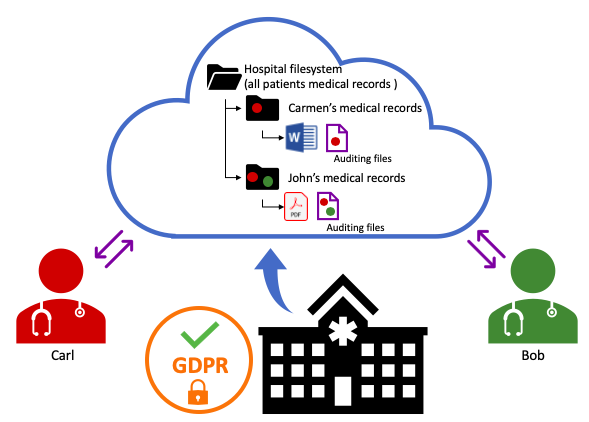
\includegraphics[width=0.75\textwidth]{images/problem/overview}
    
    \caption{Representation of the real life situation}
    \label{figure:problem:overview}
\end{figure}

\par In order to motivate our work, we are using an example linked to the healthcare domain, more precisely the hospitals. Inside an hospital, many services or doctors must share medical records of a single patient, as depicted in Figure \ref{figure:problem:overview}. How can those parties share this record without disclosing its content (to other parties) and without requiring complicated operation ? On top of that, the revocation of a doctor rights to access a specific resource, once he no longer needs it, is also a mandatory operation according GDPR.

\medbreak
\par Alongside data confidentiality, keeping track of who accessed or edited a given file is required. GDPR states that: "\textit{All EU institutions have the legal obligation to keep a central register of records of activities processing personal data}". In practice, this means that every time an authorised doctor wants to access a medical record, s/he must first explain its intention. These intents explains the purpose of the action. These purposes allows a data owner (e.g: a patient) to know who accessed his information and avoid allowed users from abusing his private data. As the purpose may itself contain confidential information, it must also be securely stored. Most of all, these intents can not be tampered with, in order to keep their accuracy. Furthermore, for a forensic purpose, it would also be interesting to spot if unauthorised user are trying to alter these data. To top it all, these intents must be easily accessible for GDPR compliance evidence.

\medbreak
\par Aside from the two above functionalities, the users (Bob and Carl) must still be able to use their usual user-space application (like Acrobat Reader, Word, PDF Reader, etc). As it is a shared filesystem, each users must be able to use it offline, while keeping the above functionalities. In the same way as Dropbox, connectivity is only useful to fetch/upload new information.


\end{document} 